
%----------------------------------------------------------------------------------------
%	PAGE 2
%----------------------------------------------------------------------------------------

\begin{frame}
\frametitle{Outline}


\begin{itemize}

  \item[$\blacksquare$] Introduction

  \vspace{5mm}

  \item[$\blacksquare$] Methodology

%  \vspace{3mm}
%
%  \item Innovated interaction screening
%
%  \vspace{3mm}
%
%  \item Post-screening variable selection

 \vspace{5mm}

 \item[$\blacksquare$] Important theoretical results

  \vspace{5mm}

  \item[$\blacksquare$] Simulations

  \vspace{5mm}

%  \item[$\blacksquare$] Discussion
%
%  \vspace{10mm}
%
%  \item Conclusions

\end{itemize}
\end{frame}

%----------------------------------------------------------------------------------------
%	PAGE 3
%----------------------------------------------------------------------------------------
\section{Introduction}
\begin{frame}
\sectionpage
%\begin{center}
%\Large\bf{Methodolody}
%\end{center}
\end{frame}

%----------------------------------------------------------------------------------------
%	PAGE 4
%----------------------------------------------------------------------------------------
\begin{frame}

\end{frame}

%----------------------------------------------------------------------------------------
%	PAGE 5
%----------------------------------------------------------------------------------------
\begin{frame}

\end{frame}

%----------------------------------------------------------------------------------------
%	PAGE 6
%----------------------------------------------------------------------------------------
\begin{frame}

\end{frame}
%----------------------------------------------------------------------------------------
%	PAGE 7
%----------------------------------------------------------------------------------------
\section{Methodology}
\begin{frame}
\sectionpage

\end{frame}


%----------------------------------------------------------------------------------------
%	PAGE 8
%----------------------------------------------------------------------------------------
\begin{frame}
\frametitle{Model setting}

\begin{itemize}

\item[$\blacksquare$] Constructing confidence intervals for the individual regression coefficients and their linear combination in the linear model,% (unobservable), %the response vector
\begin{equation}
\by = {\bX}\bbeta + \varepsilon, \qquad \mathbf{\varepsilon} \sim \mathcal{N}(\bzero,\sigma^2\bI)
\end{equation}
where $\by \in \mathbb{R}^{n}$ is a response vector, $\bX=(\bx_{1},\ldots,\bx_{p})\in \mathbb{R}^{n\times p}$ is a design matrix with columns $\bx_{j}$ and is a vector of unknown regression coefficients.
%$X\in {{\mathbb{R}}^{n\times p}}$

\vspace{3mm}

\begin{itemize}
      \item[-]  Standardize the design to $\|\bx_{j}\|^{2}_{2}=n$.

      \medskip

      \item[-] The design matrix $\bX$ is assumed to be deterministic.

\end{itemize}

\end{itemize}


\end{frame}


%----------------------------------------------------------------------------------------
%	PAGE 9
%----------------------------------------------------------------------------------------
\begin{frame}
\frametitle{Least squares estimator}
\begin{itemize}

\item[$\blacksquare$] In classical theory of linear models, the least squares estimator of an estimable regression coefficient $\bbeta_{j}$ can be written as  % (unobservable), %the response vector
\begin{equation}
\hat{\bbeta}^{(lse)}_{j} := (\bx^{\bot}_{j})\t \by /(\bx^{\bot}_{j})\t \bx_{j},
\end{equation}
where $\bx^{\bot}_{j}$ is a projection of $\bx_{j}$ to the orthogonal complement of column space of $\bX_{-j}=(\bx_{k},k\neq j)$.

\item[$\blacksquare$] The $\bx^{\perp}_{j}$ is defined by
\begin{itemize}
      \item[-] $(\bx^{\bot}_{j})\t \bx_{k}=\bzero $, for $ \forall k\neq j$.
      \medskip
      \item[-] $(\bx^{\bot}_{j})\t \bx_{j}=\|\bx_{j}\|^{2}_{2}$.

\vspace{3mm}

\end{itemize}

\end{itemize}


\end{frame}


%----------------------------------------------------------------------------------------
%	PAGE 10
%----------------------------------------------------------------------------------------
\begin{frame}
\frametitle{Problems}
\begin{itemize}

\item[$\blacksquare$] In high dimensional situation $p>n$, $rank(\bX_{-j})=n$ for all $j$. % (unobservable), %the response vector
\begin{itemize}
\item[$\blacktriangleright$] $\bx^{\bot}_{j}=\bzero$. $\hat{\bbeta}^{(lse)}_{j}$ is undefined.
\end{itemize}
\item[$\blacksquare$] We want to preserve the properties of the least squares estimator.
\begin{itemize}
\item[$\blacktriangleright$] The covariance structure of the least squares estimator:
\begin{equation}
\cov(\hat{\bbeta}^{(lse)}_{j},\hat{\bbeta}^{(lse)}_{k})=\sigma^{2} \frac{(\bx^{\bot}_{j})\t \bx^{\bot}_{k}}{\|\bx_{j}\|^{2}_{2}\|\bx_{k}\|^{2}_{2}}
\end{equation}
\end{itemize}
\item[$\blacksquare$] Motivation of LDPE:
\begin{itemize}
      \item[$\blacktriangleright$] Replace $\bx^{\bot}_{j}$ with $\bz_{j}$.
      \medskip
      \item[$\blacktriangleright$] Relaxing the constraint $\bz_{j}\t \bx_{k}=\bzero$ for $k\neq j$.
\vspace{3mm}

\end{itemize}

\end{itemize}


\end{frame}

%----------------------------------------------------------------------------------------
%	PAGE 11
%----------------------------------------------------------------------------------------
\begin{frame}
\frametitle{Bias-corrected linear estimators}
\begin{itemize}

\item[$\blacksquare$] For any $\bz_{j}$ that is not orthogonal to $\bx_{j}$, the corresponding univariate linear regression estimator satisfies
\begin{equation*}
\hat{\bbeta}^{(lin)}_{j}= \frac{\bz^{T}_{j} \by}{\bz^{T}_{j} \bx_{j}}= \beta_j + \frac{\bz_j^T \varepsilon}{\bz_j^T\bx_j}
+ \sum_{k\neq j}\frac{\bz_j^T\bx_k\beta_k}{\bz_j^T\bx_j}.
\end{equation*}
  \begin{itemize}
  \item[$\blacktriangleright$] Here,  $\hat{\bbeta}^{(lin)}_{j}$ has the same covariance structure with $\hat{\bbeta}^{(lse)}_{j}$.
  \end{itemize}
\item[$\blacksquare$] Note that the bias of $\hat{\bbeta}^{(lin)}_{j}$ is unbounded. It is impossible to have $\bz_{j}\t \bx_{k}=\bzero$ for all $k\neq j \quad (\bz_{j}\neq\bzero)$.
\end{itemize}
\end{frame}


%----------------------------------------------------------------------------------------
%	PAGE 12
%----------------------------------------------------------------------------------------
\begin{frame}
\frametitle{Low dimensional projection estimator}
\begin{itemize}

\item[$\blacksquare$] Bias correction with a non-linear initial estimator $\hat{\bbeta}^{(init)}$:
\begin{equation}
\hat{\bbeta}_{j}=\hat{\bbeta}^{(lin)}_{j} - \sum_{k \neq j}\frac{\bz_{j}\t \bx_{k} \hat{\bbeta}^{(init)}_{k} }{\bz^{T}_{j} \bx_{j}}
=\frac{\bz^{T}_{j} \by}{\bz^{T}_{j} \bx_{j}} - \sum_{k \neq j}\frac{\bz_{j}\t \bx_{k} \hat{\bbeta}^{(init)}_{k} }{\bz^{T}_{j} \bx_{j}}.
\end{equation}
   \begin{itemize}
   %\item[$\blacktriangleright$] One-step self-bias correction from $\hat{\bbeta}^{(init)}$:
   %\medskip
   \item[$\blacktriangleright$] The estimation error of $\hat{\bbeta}_{j}$:
   \begin{equation}
   \hat{\bbeta}_{j}-\bbeta_{j}=\frac{\bz^{T}_{j} \varepsilon}{\bz^{T}_{j} \bx_{j}} + \frac{\sum_{k \neq j} \bz_{j}\t \bx_{k} (\bbeta_{k} - \hat{\bbeta}^{(init)}_{k}) }{\bz^{T}_{j} \bx_{j}} \triangleq \bA + \bB.
   \end{equation}
   \item[$\blacktriangleright$] It can be viewed as a sum of noise term and bias term.
   %\vspace{3mm}
   \end{itemize}

\end{itemize}


\end{frame}


%----------------------------------------------------------------------------------------
%	PAGE 13
%----------------------------------------------------------------------------------------
\begin{frame}
\frametitle{Error analysis of LDPE$(1)$}
\begin{itemize}

\item[$\blacksquare$] The approximation error of the LDPE (Term $\bB$) can be controlled:
\begin{equation}
\Big|\sum_{k\neq j}\bz_j^T\bx_k(\beta_k-\hbeta_k^{(init)})\Big|
\le \Big(\max_{k\neq j}\big|\bz_j^T\bx_k\big|\Big)\|\hbbeta^{(init)}-\bbeta\|_1.
\end{equation}
\item[$\blacksquare$] For $\bz_{j}$, define
\begin{equation}
\label{defetatau}
\eta_j = \max_{k\neq j}\big|\bz_j^T\bx_k\big|/\|\bz_j\|_2,\qquad \tau_j = \|\bz_j\|_2/|\bz_j^T\bx_j|.
\end{equation}
   \begin{itemize}
   \item[$\blacktriangleright$] Bias factor $\eta_{j}$: $\eta_{j} \|\hat{\bbeta}^{(init)}-\bbeta\|_{1}$ controls the approximation error.
   \item[$\blacktriangleright$] Noise factor $\tau_{j}$: $\tau_{j} \sigma$ is the standard deviation of noise term.
   %\vspace{3mm}
   \end{itemize}

\end{itemize}


\end{frame}


%----------------------------------------------------------------------------------------
%	PAGE 14
%----------------------------------------------------------------------------------------
\begin{frame}
\frametitle{Error analysis of LDPE $(2)$}
\begin{itemize}

\item[$\blacksquare$] Since $\bz_{j} \t \varepsilon \sim N(\bzero, \sigma^{2} \|\bz_{j}\|^{2}_{2})$, equation $(5)$ yields
\begin{equation}
\eta_{j}\|\hat{\bbeta}^{(init)}-\bbeta\|_{1}/\sigma=o(1)\Rightarrow \tau^{-1}_{j}(\hat{\bbeta}_{j}-\bbeta_{j})\approx N(\bzero,\sigma^{2}).
\end{equation}
\item[$\blacksquare$] Confidence intervals can be constructed by condition $(8)$ and a consistent estimator of $\sigma$.
%\item[$\blacksquare$] Pick a $\bz_{j}$ with a small $\eta_{j}$ for the asymptotic normality and a small $\tau_{j}$ for efficiency of estimation.
\item[$\blacksquare$] Need to solve:
  \begin{itemize}
  \item[$\blacktriangleright$] Choose proper $\bz_{j}$.
  \item[$\blacktriangleright$] Choose $\hat{\bbeta}^{(init)}$.
% \item[$\blacktriangleright$] Estimate $\sigma$.
  \end{itemize}

\end{itemize}
\end{frame}

%----------------------------------------------------------------------------------------
%	PAGE 15
%----------------------------------------------------------------------------------------
\begin{frame}
\frametitle{How can we choose $\bz_{j}$ ?}
\begin{itemize}

\item[$\blacksquare$] Choose $\bz_{j}$ as the residual of lasso.
\begin{equation}
\bz_j = \bx_j - \bX_{-j} \hat{\gamma}_j,\
\hat{\gamma}_j = \argmin_{\bb}\Big\{\frac{\|\bx_j-\bX_{-j}\bb\|_2^2}{2n}+\lambda_j \|\bb\|_1\Big\}.
\end{equation}
\item[$\blacksquare$] $KKT$ conditions \quad  $\Rightarrow \quad |\bx_k^T\bz_j/n|\le\lambda_{j}$ for all $k \neq j$
                      $\Rightarrow \quad \eta_j\le n\lambda_j/\|\bz_j\|_2$.

\end{itemize}


\end{frame}


%----------------------------------------------------------------------------------------
%	PAGE 16
%----------------------------------------------------------------------------------------
\begin{frame}
\frametitle{How can we pick initial estimator of $\bbeta$?}
Use methods based on scaled lasso or scaled lasso-LSE to give the initial estimates ($\bbeta^{(init)}$) for LDPE and a noise level ($\sigma$) estimator for statistical inference.
\scriptsize
\begin{itemize}
\item[$\blacksquare$] The scaled lasso is a joint convex minimization method
\begin{equation}
\big\{\bbeta^{(init)},\sigma\big\} = \argmin_{\bb,\sigma}
\Big\{\frac{\|\by-\bX\bb\|_2^2}{2\sigma n} + \frac{\sigma}{2}+\lambda_0\|\bb\|_1\Big\}.
\end{equation}
\item[$\blacksquare$] The scaled lasso is biased, an alternative method scaled lasso-LSE can be applied:
\begin{equation}
\{\hat{\bbeta}^{(init)},\sigma\} = \argmin_{\bb,\sigma}
\big\{\frac{\|\by-\bX\bb\|_2^2}{2\sigma max(n-|\hat{S}^{(scl)}|,1)} + \frac{\sigma}{2}\big\}
\end{equation}
where $\hat{S}^{(scl)}$ is the set of non-zero estimated coefficients produce by scaled lasso.
%$\bb_j=\bzero \quad \forall j \not\in \hat{S}^{(scl)}$
\end{itemize}
\end{frame}


%----------------------------------------------------------------------------------------
%	PAGE 17
%----------------------------------------------------------------------------------------
\begin{frame}
\frametitle{Algorithm of LDPE}
\begin{figure}[h]
  \centering
  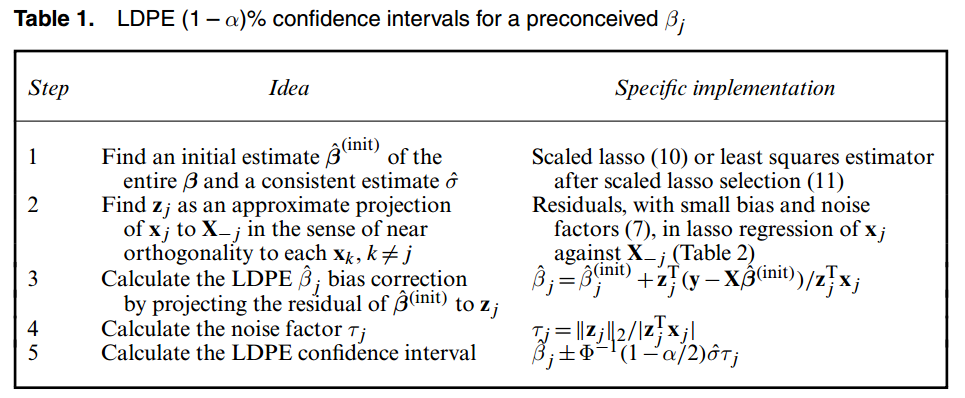
\includegraphics[width=1.0\textwidth]{./figs/Table1.png}
  \label{Table1}
\end{figure}
\end{frame}


%----------------------------------------------------------------------------------------
%	PAGE 18
%----------------------------------------------------------------------------------------
\begin{frame}
\begin{block}{Procedure of computing $\bz_{j}$}
    Along the Lasso path for regressing $\bx_j$ against $\bX_{-j}$, let
    %Here is a description of the algorithm.
    % \begin{equation}
    % \begin{aligned} 
        % \gamma_j(\lambda) &= \mathop{\arg\min}_{\bb} \{\|\bx_j -\bX_{-j}\bb\|_2^2/(2n) + \lambda\|\bb\|_1\}, \\
        % \bz_j(\lambda)   &= \bx_j-\bX_{-j}\gamma_j(\lambda), \\
        % \eta_j(\lambda) &= \max_{k\neq j}  |\bx_k^T\bz_j(\lambda)|/\|\bz_j(\lambda)\|_2, \\
        % \tau_j(\lambda)  &=  \|\bz_j(\lambda)\|_2/|\bx_j^T\bz_j(\lambda)|, 
    % \end{aligned}
    % \end{equation}
    be the coefficient estimator $\gamma_j$, residual $\bz_j$, the bias factor $\eta_j$, and
    the noise factor $\tau_j$, as functions of $\lambda$.
\end{block}
\begin{gather}
    \gamma_j(\lambda) = \mathop{\arg\min}_{\bb} \{\|\bx_j -\bX_{-j}\bb\|_2^2/(2n) + \lambda\|\bb\|_1\}, \notag \\
    \bz_j(\lambda)   = \bx_j-\bX_{-j}\gamma_j(\lambda), \notag \\
    \eta_j(\lambda) = \max_{k\neq j}  |\bx_k^T\bz_j(\lambda)|/\|\bz_j(\lambda)\|_2, \notag \\
    \tau_j(\lambda)  =  \|\bz_j(\lambda)\|_2/|\bx_j^T\bz_j(\lambda)|, 
\end{gather}
\end{frame}

%----------------------------------------------------------------------------------------
%	PAGE 19
%----------------------------------------------------------------------------------------
\begin{frame}
\frametitle{Computation of $\bz_{j}$}
\begin{figure}[h]
  \centering
  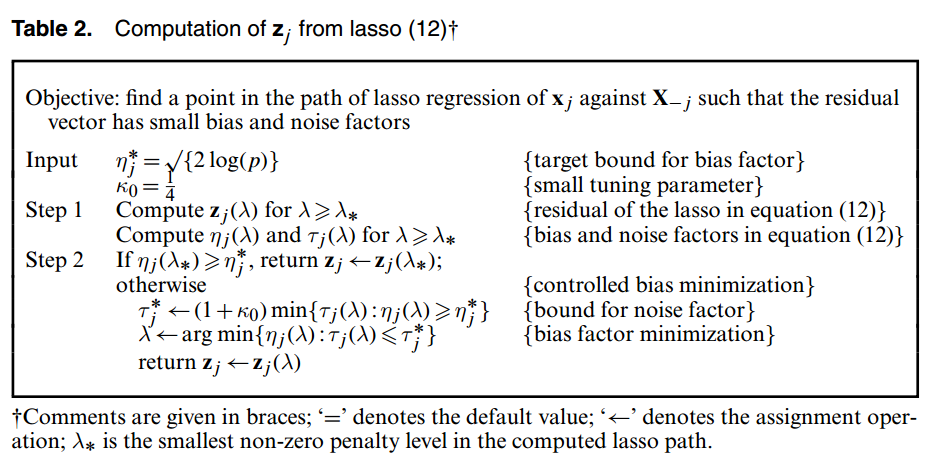
\includegraphics[width=1.0\textwidth]{./figs/Table2.png}
  \label{Table2}
\end{figure}
\end{frame}

%----------------------------------------------------------------------------------------
%	PAGE 20
%----------------------------------------------------------------------------------------
\begin{frame}
\begin{block}{Proposition 1}
\scriptsize
(a) In the Lasso path, $\|\bz_j(\lambda)\|_2$, $\eta_j(\lambda)$, and $\sigma_j(\lambda)$
are nondecreasing functions of $\lambda$, and $\tau_j(\lambda)\le 1/\|\bz_j(\lambda)\|_2$. Moreover,
$\gamma_j(\lambda)\neq 0$ implies $\eta_j(\lambda)=\lambda n/\|\bz_j(\lambda)\|_2$. \\

(b) Let $\lambda_{univ}=\sqrt{(2/n)\log p}$. Then,
\begin{equation}
\sigma_j(C\lambda_{univ})>0 \hbox{ iff } \{\lambda>0: \eta_j(\lambda) \le C\sqrt{2\log p}\}\neq \emptyset,
\end{equation}
    and in this case, the algorithm in Table 2 provides
\begin{gather}
\eta_{j}\leq \eta_j^*\le (1\vee C)\sqrt{2\log p},\\
\tau_j\le n^{-1/2}(1+\kappa_0)/\hat{\sigma}_j(C\lambda_{univ}).
\end{gather}
    Moreover, when $\bz_j(0)=\bx_j^\perp =0$, $\eta_j(0+) \inf\{\|\gamma_j\|_1: \bX_{-j}\gamma_j=\bx_j\}=\sqrt{n}$.\\
(c) Let $0<a_0<1\leq C_0<\infty$. Suppose that for $s=a_0n/\log p$
\begin{equation*}
\inf_{\delta}\sup_{\bbeta}\Big\{\|\delta(\bX,\by) - \bbeta\|_2^2: \by=\bX\bbeta,
\hbox{$\sum_{j=1}^p$} \min(|\beta_j|/\lambda_{univ},1)\le s+1 \Big\}\le 2C_0s(\log p)/n.
\end{equation*}
\end{block}
\end{frame}


%----------------------------------------------------------------------------------------
%	PAGE
%----------------------------------------------------------------------------------------
\begin{frame}
\frametitle{Restricted LDPE}
\begin{itemize}
    \item Why use restircted lasso relaxation for $bz_j$?
    The summands with larger absolute correlation $|\bx_j^T\bx_k/n|$ are likely to have a greater contribution to the bias due to initial estimation error $|\bbeta^{(init)}_k-\beta_k|$.
    \item How to implement restricted LDPE(RLDPE)?
    Force smaller $|\bz_j^T\bx_k/n|$ for large $|\bx_j^T\bx_k/n|$ with a weighted relaxation:
    \begin{equation}
    \bz_j = \bx_j - \bX_{-j}\gamma_j,\qquad \gamma_j = \mathop{\arg\min}_{\bb}\left\{\frac{\|\bx_j-\bX_{-j}\bb\|_2^2}{2n} + \lambda_j\sum_{k\neq j}w_k|b_k|\right\},
    \end{equation}
    with $w_k$ being a decreasing function of the absolute correlation $|\bx_j^T\bx_k/n|$.
    \item[$\blacksquare$] Simply set $w_k=0$ for large $|\bx_j^T\bx_k/n|$ and $w_k=1$ for other $k$ in the RLDPE.
    
\end{itemize}
\end{frame}


%----------------------------------------------------------------------------------------
%	PAGE 21
%----------------------------------------------------------------------------------------
\section{Important theoretical results}
\begin{frame}
\sectionpage
\end{frame}


%----------------------------------------------------------------------------------------
%	PAGE 3.1 22
%----------------------------------------------------------------------------------------
\begin{frame}
\begin{block}{Conditions}
\scriptsize
    Let $\lambda_{univ}=\sqrt{(2/n)\log p}$. Suppose the model $(1)$ holds with a vector $\bbeta$ satisfying the following capped-$\ell_1$ sparsity condition:
\vspace{1mm}
\begin{equation}
\label{con19}
\setlength{\abovedisplayskip}{3pt} %%% 3pt 个人觉得稍妥,可自行设置
\setlength{\belowdisplayskip}{3pt}
\sum_{j=1}^p \min\big\{|\beta_j|/(\sigma \lambda_{univ}),1\big\} \leq s.
\end{equation}
This condition holds if $\bbeta$ is $\ell_0$ sparse with $\|\bbeta\|_0 \leq s$ or $\ell_q$ sparse with $\|\bbeta\|_q^q/(\sigma\lambda_{univ})^q \leq s$, $0<q \leq 1$.
    Let $\sigma^*=\|\varepsilon\|_2/\sqrt{n}$. A generic condition we impose on the initial estimator is
\vspace{1mm}
\begin{equation}
\label{con20}
P\Big\{ \|\hat{\bbeta}^{(init)} - \bbeta\|_1 \geq C_1 s \sigma^*\sqrt{(2/n)\log(p/\epsilon)}\Big\} \leq \epsilon
\end{equation}
for a certain fixed constant $C_1$ and all $\alpha_0/p^2 \leq \epsilon \leq 1$,
where $\alpha_0\in (0,1)$ is a preassigned constant.
We also impose a similar generic condition on an estimator $\hat{\sigma}$ for the noise level:
\vspace{1mm}
\begin{equation}
\label{con21}
P\Big\{ |\sigma/\sigma^* - 1 | \geq C_2 s (2/n)\log(p/\epsilon) \Big\} \leq \epsilon, \forall \alpha_0/p^2 \leq \epsilon \leq 1,
\end{equation}
with a fixed $C_2$.
%We use the same $\eps$ in (\ref{ell_1-err-bd}) and (\ref{sigma-err-bd}) without much loss of generality.
\end{block}
\end{frame}

%----------------------------------------------------------------------------------------
%	PAGE 3.1 23
%----------------------------------------------------------------------------------------
\begin{frame}
\begin{block}{Theorem 1}
\scriptsize
Let $\hat{\beta}_j$ be the LDPE with an initial estimator $\hat{\bbeta}^{(init)}$.
%Let $\eta_j=\max_{k\neq j}|\bx_k^T\bz_j|/\|\bz_j\|_2$, $\tau_j=\|\bz_j\|_2/|\bx_j^T\bz_j|$,
%$\max(\eps_n',\eps_n'')\to 0$, and $\eta^*>0$.
Let $\eta_j$ and $\tau_j$ be the bias and noise factors in (\ref{defetatau}),
$\sigma^*=\|\varepsilon\|_2/\sqrt{n}$,
$\max(\epsilon_n',\epsilon_n'')\to 0$, and $\eta^*>0$.
Suppose (\ref{con20}) holds with $\eta^*C_1s\sqrt{(2/n)\log(p/\epsilon)} \leq \epsilon_n'$.
If $\eta_j \leq \eta^*$, then
\begin{equation}
\label{thm22}
P\Big\{ \big|\tau_j^{-1}(\hat{\beta}_j - \beta_j) - \bz_j^T \varepsilon/\|\bz_j\|_2\big|
> \sigma^* \epsilon_n'\Big\} \leq \epsilon.
\end{equation}
If in addition (\ref{con21}) holds with $C_2 s (2/n)\log(p/\epsilon)\leq \epsilon_n''$, then for all
$t\ge (1+\epsilon_n')/(1-\epsilon_n'')$,
\begin{equation}
\label{thm23}
P\Big\{|\beta_j - \beta_j| \ge \tau_j\sigma t\Big\}\le 2\Phi_{n-1}(-(1-\epsilon_n'')t+\epsilon_n')+2\epsilon,
\end{equation}
where $\Phi_n(t)$ is the student-t distribution function with $n$ degrees of freedom.
Moreover, for the covariance matrix $\bV$ in and all fixed $m$,
\begin{equation}
\label{thm24}
\lim_{n\to\infty}
\inf_{\ba\in \mathscr{A}_{n,p,m}}P\Big\{\big|\ba^T\hat{\bbeta} - \ba^T\bbeta\big|
\leq \hat{\sigma}\Phi^{-1}(1-\alpha/2)(\ba^T\bV\ba)^{1/2}\Big\} = 1-\alpha,
\end{equation}
where $\Phi(t) = P\{ N(0,1)\le t\}$ and
$\mathscr{A}_{n,p,m}=\{\ba: \|\ba\|_0 \leq m, \max_{j \leq p}|a_j|\eta_j\leq \eta^*\}$.
\end{block}
\medskip   
    This allows us to write the LDPE as an approximate Gaussian sequence
\begin{equation}
\label{Gauseq}
\beta_j = \beta_j + N(0,\tau_j^2\sigma^2) + o_P(\tau_j\sigma).
\end{equation}
\end{frame}


%----------------------------------------------------------------------------------------
%	PAGE 3.3 24
%----------------------------------------------------------------------------------------
\begin{frame}
    \frametitle{Thresholded LDPE}
    %\begin{itemize}
    %\item[$\blacksquare$] 
        From $Theorem 1$, the $\hat{\bbeta}_{j}$ can be viewed as an approximate Gaussian sequence. The approximately normal sequence is not spare but can be thresholded.
        Using either the hard or the soft thresholding method:
        
        lost function group
    %    \begin{itemize}
    %    \item[$\blacktriangleright$] 
    
    \begin{equation}\label{TLDPE}
    \hat{\bbeta}^{(thr)}_{j}=
    \left\{
            \begin{aligned}%{lr}
            & \hat{\bbeta}_{j} I(|\hat{\bbeta}_{j}|>\hat{t}_{j}),   \\
            & sgn(\hat{\bbeta}_{j})(|\hat{\bbeta}_{j}|-\hat{t}_{j})^{+}, \\
            \end{aligned}
    \right.
    \end{equation}
    with
    \begin{equation*}
    \hat{S}^{(thr)}=\{j:|\hat{\bbeta}_{j}|>\hat{t}_{j}\}
    \end{equation*}
    
    %\end{itemize}
    
\end{frame}


%----------------------------------------------------------------------------------------
%	PAGE $3.3  25
%----------------------------------------------------------------------------------------
\begin{frame}
\begin{block} {Theorem 3}
\scriptsize
    Let $L_0=\Phi^{-1}(1-\alpha/(2p))$, $\tilde{t}_j = \tau_j\sigma L_0$, and
$\hat{t}_j = (1+{c}_n)\sigma\tau_j L_0$ with positive constants $\alpha$ and ${c}_n$. Suppose
condition (queshao) holds with $\eta^*C_1s/\sqrt{n}\leq \epsilon_n'$, $\max_{j\leq p}\eta_j\leq \eta^*$, and
\begin{equation}
P\Big\{\frac{(\sigma/\sigma)\vee(\sigma/\sigma) -1+\epsilon_n'\sigma^*/(\sigma\wedge \sigma)}
{1-(\sigma/\sigma-1)_+ } > {c}_n\Big\} \leq 2\epsilon.
\end{equation}
    Let $\bbeta^{(thr)} = (\beta_1^{(thr)},\ldots,\beta_p^{(thr)})^T$ be the {soft} thresholded LDPE
with these $\hat{t}_j$.
Then, there is an event $\Omega_n$ with $P\{\Omega_n^c\} \leq 3 \epsilon$ such %that
%\begin{equation}
%E\|\bbeta^{( thr)} - \bbeta\|_2^2I_{\Omega_n} \leq \sum_{j=1}^p \min\{\beta_j^2,\tau_j^2\sigma^2(L_0^2(1+2{c}_n)^2+1)\} +(\eps L_n/p)\sigma^2\sum_{j=1}^p\tau_j^2,
%\end{equation}
where $L_n = 4/L_0^3+4{c}_n/L_0+12{c}_n^2L_0$.
Moreover, with at least probability $1-\alpha - 3\epsilon$,
\begin{equation}
\{j: |\beta_j|> (2+2{c}_n)\tilde{t}_j\} \subseteq \hat{S}^{(thr)} \subseteq \{j:\beta_j\neq 0\}.
\end{equation}
\end{block}
\end{frame}

%----------------------------------------------------------------------------------------
%	PAGE $3.3 compare
%----------------------------------------------------------------------------------------
\begin{frame}
\frametitle{Thresholded LDPE  VS.  Lasso}
\begin{itemize}
\item[$\blacksquare$] Uniform signal strength condition
\medskip
\item[$\blacksquare$] Varaible selection
\medskip
\item[$\blacksquare$] Thresholded quantities
\medskip
\item[$\blacksquare$] $\ell_2$ estimation error
%  \begin{itemize}
%  \item[$\blacktriangleright$] Make no assumption of uniform signal strength condition.
%  \item[$\blacktriangleright$] Large $|\bbeta_{j}|$ are selected by the thresholded LDPE and $\bbeta_{j}=\bzero$ are not select in the presence of small $|\bbeta_{j}|\neq\bzero$.
%  \item[$\blacktriangleright$] Threshold on approximately Gaussian sequence, requires only univariate analysis.
%  \item[$\blacktriangleright$] The order of the $\ell_2$ error bound is slightly sharper than the typical order of $\|\bbeta\|_0\sigma^2\lambda_{univ}^2$ or $\sigma\lambda_{univ}\sum_{j=1}^p \min\big\{|\beta_j|, \sigma\lambda_{univ}\big\}$
%  \end{itemize}

%\bigskip

%\item[$\blacksquare$] Lasso and other regularized methods
%  \begin{itemize}
%  \item[$\blacktriangleright$] Variable selection consistency requires the uniform signal strength condition.
%  \item[$\blacktriangleright$] Can not guaranteed to select correctly variables with large $|\bbeta_{j}|$ or $\bbeta_{j}=\bzero$ in the presence of small $|\bbeta_{j}|\neq\bzero$.
%  \item[$\blacktriangleright$] Thresholded quantities:Thresholding is applied to the gradient $\bX^T(\by-\bX\bbeta)/n$ via the Karush-Kuhn-Tucker-type condition, leading to more complicated nonlinear multivariate analysis.
% \item[$\blacktriangleright$] Rate optimal in the maximum $\ell_2$ estimation loss for many classes of sparse $\bbeta$

%\end{itemize}

\end{itemize}
\end{frame}

%----------------------------------------------------------------------------------------
%	PAGE
%----------------------------------------------------------------------------------------
\section{Simulation}
\begin{frame}
\sectionpage
\end{frame}

%----------------------------------------------------------------------------------------
%	PAGE
%----------------------------------------------------------------------------------------
\begin{frame}
\frametitle{Simulation result}
\begin{figure}[h]
  \centering
  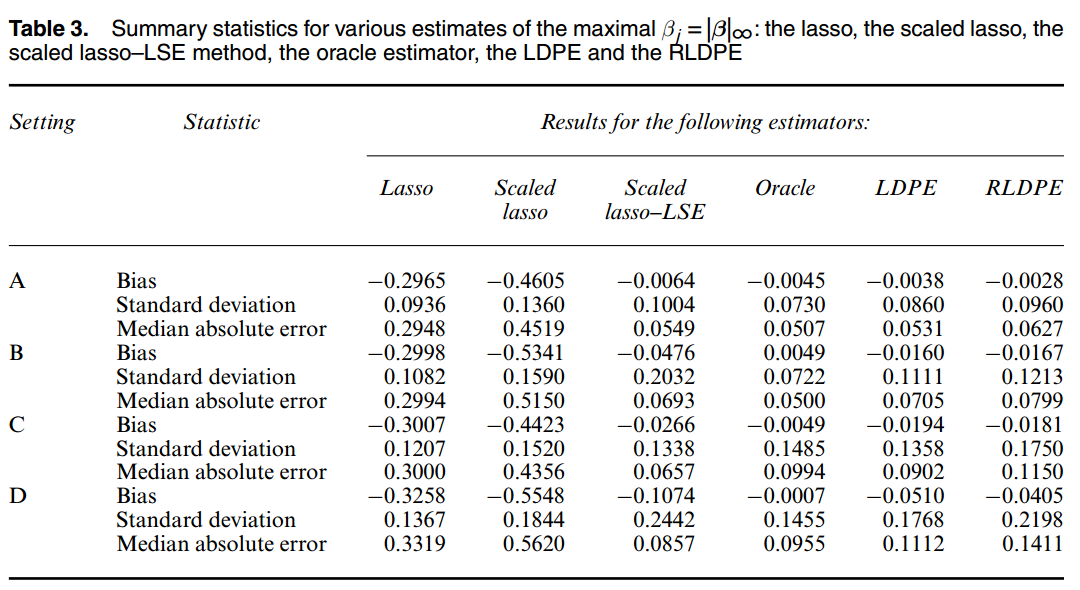
\includegraphics[width=1.0\textwidth]{./figs/Table3.png}
  \label{Table1}
\end{figure}
\end{frame}


%----------------------------------------------------------------------------------------
%	PAGE
%----------------------------------------------------------------------------------------
\begin{frame}
\frametitle{Simulation result}
\begin{figure}[h]
  \centering
  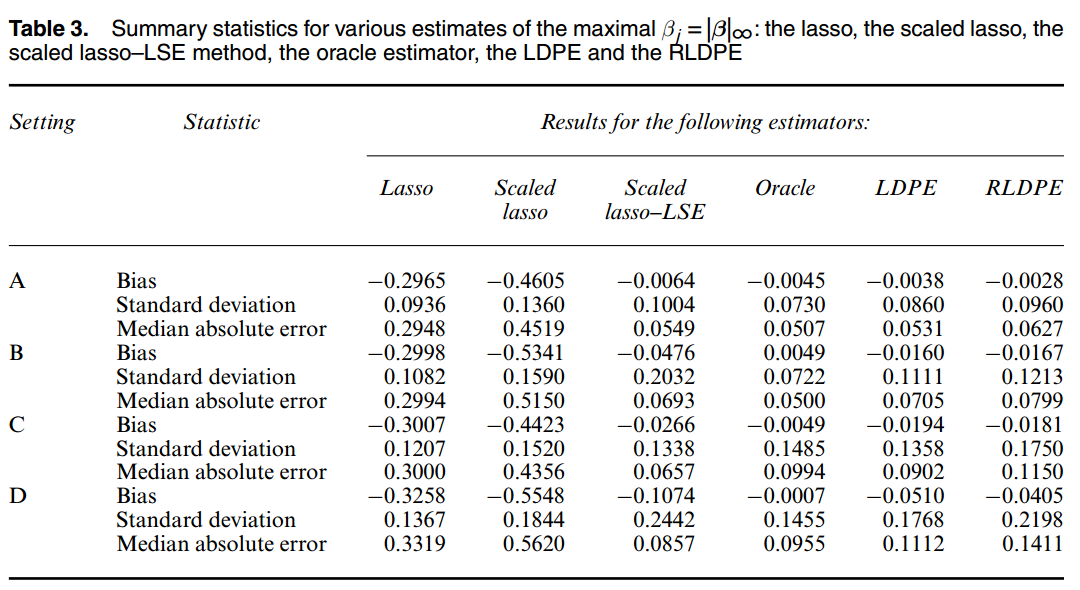
\includegraphics[width=1.0\textwidth]{./figs/Table3.png}
  \label{Table1}
\end{figure}
\end{frame}
